\section{Predicció amb Models Lineals o Quadràtics}
En primer lloc es discutirà els models lineals o quadràtics que s'ha emprat en aquesta pràctica: K nearest neighbors, LDA , QDA i SVM quadratic.
\subsection{K nearest neighbors}
El paràmetre principal per a KNN és $k$, el nombre de veïns que ha de tenir en compte l'algorisme. Per trobar la $k$ més precisa s'ha usat \textit{Leave-One-Out Cross-Validation}(LOOCV) per provar quin valor de $k$ s'ajusta millor al model i dóna un error menor.
\begin{table}[H]
	\centering
	\def\arraystretch{1.2}
	\begin{tabular}{|rrr|}
		\hline
		k  & Accuracy & Kappa \\
		\hline
		\textbf{1}  &  \textbf{0,9541919} & \textbf{0,9523578} \\
		2  &  0,9447021 & 0,9424881 \\
		3  &  0,9494827 & 0,9474599 \\
		4  &  0,9481270 & 0,9460500 \\
		5  &  0,9490546 & 0,9470148 \\
		6  &  0,9451302 & 0,9429332 \\
		7  &  0,9419194 & 0,9395936 \\
		8  &  0,9402783 & 0,9378867 \\
		9  &  0,9384945 & 0,9360312 \\
        10 &  0.9372815 & 0.9347697 \\
        11 &  0.9349269 & 0.9323209 \\
        12 &  0.9326436 & 0.9299463 \\
        13 &  0.9305744 & 0.9277941 \\
        14 &  0.9293614 & 0.9265327 \\
        15 &  0.9284338 & 0.9255680 \\
		\hline
	\end{tabular}
	\caption{Precisió de diferents valors de k utilitzant LOOCV.}
	\label{tab:nnet_k}
\end{table}
Com es pot veure a la taula \ref{tab:nnet_k} el valor que dóna un error menor és quan el valor de $k$ és 1.
Un cop ajustat el valor de k s'entrena el model i es comprova el seu error amb el conjunt de prova. Els resultats obtinguts de precisió 95.42\%, és a dir, un error de 4.58\%. En la taula~\ref{mck} la matriu de confusió.

\begin{figure}[H]
    \centering
    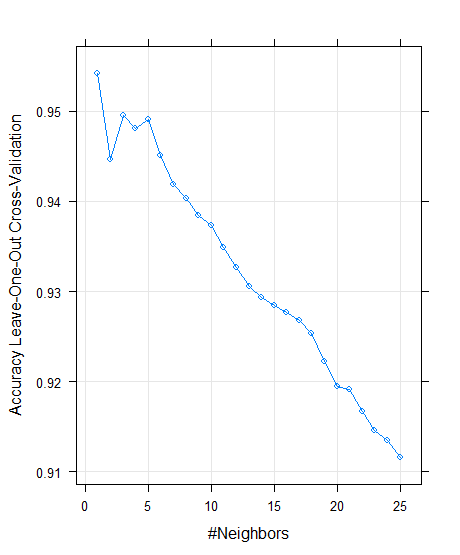
\includegraphics[height=0.8\textwidth]{img/plotmodelknn.png}
    \caption{Precisió de CV en funció de k}
    \label{fig:knnmodel}
\end{figure}
Tal com es pot veure a la Figura \ref{fig:knnmodel} a mesura que s'augmenta $k$ la precisió del model disminueix progressivament, excepte pels valors de 3 a 7 que té més variància encara que el punt amb més precisió és $k=1$.

\subsection{SVM quadràtic}
Per a classificar mitjançant Màquines de Vectors de Suport(SVM) s'ha escalat les dades, s'utilitza \textit{5-fold Cross-Validation} per tal de trobar el millor valor pel paràmetre $C$, utilitzant un grau de 2 per tal de que sigui SVM quadràtic. El paràmetre $C$ serveix per reduir el sobreajust. Usem a \textit{Cross-Validation} els possibles valors de $C$ com: 0.01,0.1,1,10,100. Els resultats obtinguts són els següents:
\begin{table}[H]
	\centering
	\def\arraystretch{1.2}
	\begin{tabular}{|rrr|}
		\hline
		C  & Accuracy & Kappa \\
		\hline
		0.01  &  0.9360691 & 0.9335089 \\
		\textbf{0.1}  &  \textbf{0.9563326} & \textbf{0.9545840} \\
		1  &  0.9528362 & 0,9509477 \\
		10  &  0,9513383 & 0,9493899 \\
		100  &  0,9513383 & 0,9493899 \\
		1000  &  0,9513383 & 0,9493899 \\
		\hline
	\end{tabular}
	\caption{Evolució de la precisió de diferents valors de C utilitzant 5-fold Cross-Validation.}
	\label{tab:nnet_k}
\end{table}
Com es pot observar el valor de $C$ que ens dóna \textit{Cross-Validation} com a optim és 0.1 amb molt poca diferencia amb 1 (diferencia en el quart decimal). Un cop ajustat el valor de $C$ es prediu el conjunt de prova amb la $C$ abans trobada, el resultat obtingut és d'una precisió de 95.86\% que vol dir un error de 4.14\%. A continuació es mostra la matriu de confusió utilitzada per calcular l'error.


\begin{figure}[H]
    \centering
    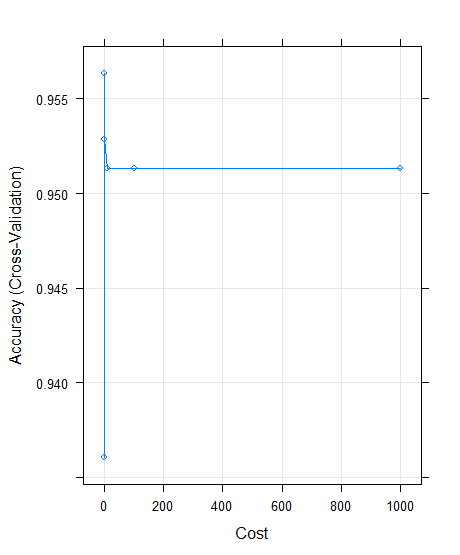
\includegraphics[height=0.8\textwidth]{img/plotsvmqmodel.png}
    \caption{Evolució de la precisió de CV en funció de C}
    \label{fig:svmqmodel}
\end{figure}   

\subsection{LDA}
En aquesta secció s'obté un model LDA i a continuació es comprova el model mitjançant \textit{Leave-One-Out Cross-Validation}(LOOCV). L'error de LOOCV és de 29.80\%. Seguidament es mostra la matriu de confusió utilitzada per calcular l'error de prova.

El model aconsegueix un 70.04\% d'encert en el conjunt de dades de prova.

\subsection{QDA}
Per QDA també utilitzem \textit{Leave-One-Out Cross-Validation}(LOOCV) per tal de calcular el model òptim. L'error de LOOCV és de 11.54477. A continuació es mostra la respectiva matriu de confusió al calcular l'error de test.



El model aconsegueix un 88.47\% d'encert en el conjunt de dades de prova.

Després de veure els resultats de LDA i QDA és hora de comparar-los. El mètode quadràtic és més precís que el lineal amb un error de 11.52\% contra un error de 29.80\%. 
